\documentclass[11pt,a4paper,twoside]{tesis}
% SI NO PENSAS IMPRIMIRLO EN FORMATO LIBRO PODES USAR
%\documentclass[11pt,a4paper]{tesis}

\usepackage{graphicx}
\usepackage{adjustbox}
\usepackage{amssymb}
\usepackage{amsmath}
\usepackage{amsthm}
\usepackage{booktabs}
\usepackage[tables]{xcolor}
\usepackage[obeyFinal]{easy-todo}
\usepackage{colortbl}
\usepackage[utf8]{inputenc}
\usepackage[spanish]{babel}
\usepackage[left=3cm,right=3cm,bottom=3.5cm,top=3.5cm]{geometry}
\usepackage{xspace}

\begin{document}

%%%% CARATULA
% Comentar y descomentar según corresponda
\def\titulo{Licenciatura\xspace}

\def\autor{Juan Manuel Pérez}
\def\tituloTesis{Métricas de mimetización acústico-prosódica en hablantes y su relación con rasgos sociales de diálogos}
\def\runtitulo{\tituloTesis}
\def\director{Agustín Gravano}
\def\codirector{Ramiro H. Gálvez}
\def\lugar{Buenos Aires, 2016}
\newcommand{\absentrainment} {\emph{unsigned entrainment}\xspace}
\newcommand{\fwentrainment}[1] {\mathcal{E}_{#1}}

\newcommand{\entrainment} {\emph{entrainment}\xspace}
\newcommand{\disentrainment} {\emph{disentrainment}\xspace}
\newcommand{\ap} {acústico-prosódicas\xspace}

\newcommand{\TAMA} {\emph{TAMA}\xspace}
%%% Variables A/P
\newcommand{\apvar}[1]{\emph{#1}\xspace}

\newcommand{\ENGMAX} {\apvar{Int Max}}
\newcommand{\ENGMEAN} {\apvar{Int Mean}}
\newcommand{\FOMAX} {\apvar{F0 Max}}
\newcommand{\FOMEAN} {\apvar{F0 Mean}}
\newcommand{\NOISETOHARMONICS} {\apvar{NHR}}
\newcommand{\SYLAVG} {\apvar{Sílabas/seg}}
\newcommand{\PHONAVG} {\apvar{Fonemas/seg}}
\newcommand{\LOCALSHIMMER} {\apvar{Shimmer}}
\newcommand{\LOCALJITTER} {\apvar{Jitter}}


%%% variables sociales

\newcommand{\socialvariable}[1] {\emph{#1}\xspace}
\newcommand{\svcontributes} {\socialvariable{contributes-to-completion}}
\newcommand{\svclear} {\socialvariable{making-self-clear}}
\newcommand{\svengaged} {\socialvariable{engaged-with-game}}
\newcommand{\svplanning} {\socialvariable{planning-what-to-say}}
\newcommand{\svencourages} {\socialvariable{gives-encouragement}}
\newcommand{\svdifficult} {\socialvariable{difficult-for-partner-to-speak}}
\newcommand{\svbored} {\socialvariable{bored-with-game}}
\newcommand{\svdislikes} {\socialvariable{dislikes-partner}}

%%% Time series

\newcommand{\varnorm}[1] {
    (#1_t - \mu_{#1})
}

%%% Regresión and stuff
\newcommand{\estslope} {\widehat{\beta_2}}
\newcommand{\estintercept} {\widehat{\beta_1}}
\newcommand{\softhl} {\rowcolor[gray]{.88}}
\newcommand{\hl} {\rowcolor[gray]{.80}}
\newcommand{\stronghl} {\rowcolor[gray]{.75}}

% psl is "Positive Slope"
\newcommand{\psl} { $+$ }
\newcommand{\ppsl} { $++$ }
\newcommand{\pppsl} { $+++$ }

% nsl stands for "Negative SLope"
\newcommand{\nsl} { $-$ }
\newcommand{\nnsl} { $--$ }
\newcommand{\nnnsl} { $---$ }


\input{caratula}

%%%% ABSTRACTS, AGRADECIMIENTOS Y DEDICATORIA
\frontmatter
\pagestyle{empty}

\chapter*{\runtitulo}

Los sistemas de diálogo humano-computadora son cada vez más frecuentes, y sus aplicaciones comprenden una amplia gama de rubros: desde aplicaciones móviles, motores de búsqueda, juegos, hasta tecnologías de asistencia para ancianos y discapacitados. Si bien es cierto que estos sistemas logran captar buena parte de la dimensión lingüística de la comunicación humana, tienen un déficit importante a la hora de procesar y transmitir el aspecto superestructural de la comunicación oral, que radica en el intercambio de afecto, emociones, actitudes y otras intenciones de los participantes.

El \emph{entrainment} (mimetización) es un fenómeno inconsciente que se manifiesta a través de la adaptación de posturas, forma de hablar, gestos faciales y otros comportamientos entre dos o más interactores. A su vez, la ocurrencia de esta mimetización está fuertemente emparentada con el sentimiento de empatía y compenetración entre los participantes. En nuestro caso, nos es de interés el \emph{entrainment} sobre las variables acústico-prosódicas, como el tono, intensidad, y otras.

En el presente trabajo, nos proponemos explorar y refinar una métrica del entrainment acústico-prosódico definida en trabajos previos. Analizamos la relación entre los valores obtenidos y las percepciones sociales que terceros tienen sobre las conversaciones, en un corpus de diálogos orientados a tareas en inglés.

\bigskip

\noindent\textbf{Palabras claves:} Procesamiento del Habla, Series de Tiempo, Entrainment, Regresión Lineal

\hfill \textit{A mis amigos.}

\hfill \textit{A mis compañeros de la Facultad, con los que tanto remamos.}

\hfill \textit{A mi familia, que me acompañaron.}

\tableofcontents

\mainmatter
\pagestyle{headings}

%%% Macros

%%%% ACA VA EL CONTENIDO DE LA TESIS
\chapter{Introducción}
\begin{frame}
  \frametitle{Sistemas de diálogo Humano-Computadora}

  \begin{enumerate}[<+->]
    \item Sistemas actuales
    \item Bien en la parte lingüística de la comunicación: entender y transmitir mensajes estructuralmente correctos.
    \item Mal en la parte superestructural: intercambio de emociones, actitudes, etc.
    \item El presente trabajo trata de hacer un (pequeño) aporte sobre el análisis de la ``naturalidad'' de las conversaciones.
  \end{enumerate}
\end{frame}


\begin{frame}
  \begin{columns}
    \column{0.5\textwidth}
    \frametitle{Ejemplos de ``falta de naturalidad''}
    \begin{enumerate}
      \item Sistemas de llamadas comerciales
      \item Siri, Google Now
      \item Otros?
    \end{enumerate}
    \column{0.5\textwidth}
    \begin{figure}
      \includegraphics[scale=0.25]{images/hal.jpg}
    \end{figure}
  \end{columns}
\end{frame}


\begin{frame}
  \frametitle{Prosodia}
  \framesubtitle{Definir acá qué es la prosodia aproximadamente}

\end{frame}



\begin{frame}
  \frametitle{Entrainment}

  \begin{enumerate}
    \item Fenómeno ubícuo en la comunicación
    \item Ocurre a varios niveles
    \item Largamente estudiado en psicología de comportamiento (referencias)
    \item (ya está, la próxima conversación que tengan afuera de acá van a chequear ésto)
  \end{enumerate}
\end{frame}

\begin{frame}
  \frametitle{¿Y cómo lo medimos?}
  La definición de entrainment hasta acá vista es heurística! ¿Cómo definimos una medida para esto?

  Vamos a explorar una métrica definida en trabajos anteriores, pulirla un poco, y verificar que efectivamente capture ciertas características del entrainment.

  ¿Cómo? Usando un corpus con anotaciones sociales


\end{frame}



\chapter{Antecedentes}
\begin{frame}
  \frametitle{Otras métricas}

  \begin{itemize}
    \item La mimetización es un fenómeno tanto lineal: se va acentuando a lo largo de la conversación
    \item Pero también es un fenómeno dinámico: va variando localmente a lo largo de la conversación.
  \end{itemize}

  Muchas métricas sólo toman la parte global, dividiendo la conversación en 2 o más partes y luego calculando la diferencia entre las medias de las diferentes variables acústicas en cada sección.
\end{frame}


\begin{frame}
  \frametitle{Problema del alineamiento de tiempo}

  \begin{figure}[t]
    
\includegraphics[scale=0.40]{images/conversation_turns.pdf}
  \end{figure}

  \begin{itemize}
    \item ¿Cómo comparamos los diferentes turnos de una conversación?
    \item Comparar uno a uno es un enfoque simplista y no representativo de la realidad
  \end{itemize}
\end{frame}

\begin{frame}
  \frametitle{Método TAMA}
\end{frame}




\chapter{Materiales y Método}
\subsection{Corpus}
\begin{frame}
  \frametitle{Columbia Games Corpus}
  \framesubtitle{Descripción}
  \begin{columns}
    \column{0.35\textwidth}
      \begin{figure}
        \includegraphics[width=\textwidth]{images/columbia_games_color.jpg}
      \end{figure}

    \column{0.65\textwidth}

    \begin{itemize}
      \item Desarrollado por Agustín Gravano para su tesis doctoral.
      \item Corpus de conversaciones diádicas en Inglés Norteamericano
      \item 12 sesiones con 14 tareas/juegos cada una.
      \item En cada sesión, se sentó a dos participantes en una cabina profesional de grabación, y una cortina opaca colgando entre ellos para evitar la comunicación visual.
      \item Los participantes contaron con computadoras a través de las cuales interactuaban mediante juegos.
    \end{itemize}
  \end{columns}
\end{frame}


\begin{frame}
  \frametitle{Columbia Games Corpus}
  \framesubtitle{Anotaciones sociales}

  Cinco anotadores escucharon el audio correspondiente a una tarea del juego y respondieron a varias preguntas sobre los sujetos:


\begin{table}
\adjustbox{max width=0.8\textwidth}{
\begin{tabular}{|l|l|}
  \hline

  \textbf{Nombre} & \textbf{Pregunta} \\
  \hline

  \svcontributes &  ¿el sujeto contribuye para el éxito del equipo?  \\ \hline
  \svengaged &  ¿el sujeto parece comprometido con el juego? \\ \hline
  \svclear &  ¿el sujeto se expresa correctamente? \\ \hline
  \svplanning &  ¿el sujeto piensa lo que va a decir? \\ \hline
  \svencourages &  ¿el sujeto alienta a su compañero? \\ \hline
  \svdifficult &  ¿el sujeto le hace difícil hablar a su compañero? \\ \hline
  \svbored &  ¿el sujeto está aburrido con el juego? \\ \hline
  \svdislikes &  ¿al sujeto no le agrada su compañero? \\ \hline
\end{tabular}
}
\end{table}

De cada una de estas preguntas obtenemos un puntaje de 0 a 5, para cada hablante de cada tarea.
\end{frame}


\begin{frame}
\frametitle{Extracción de features acústico-prosódicas}

Usando el software Praat \footnote{http://www.fon.hum.uva.nl/praat/} se extrajeron las variables acústico-prosódicas para cada segmento de habla

\begin{table}
\adjustbox{max width=0.8\textwidth}{
\centering
\begin{tabular} {|c|c|}
  \hline
  Variable & Descripción \\
  \hline
  \FOMEAN & Valor medio de la frecuencia fundamental \\\hline
  \FOMAX  & Valor máximo de la frecuencia fundamental \\\hline
  \ENGMEAN & Valor medio de la intensidad \\\hline
  \ENGMAX & Valor máximo de la intensidad \\\hline
  \NOISETOHARMONICS & Noise-to-harmonics ratio \\\hline
  \LOCALSHIMMER & Shimmer medido \\\hline
  \LOCALJITTER  & Jitter medido \\\hline
  \SYLAVG & Cantidad de sílabas por segundo \\\hline
  \PHONAVG & Cantidad de fonemas por segundo \\\hline
\end{tabular}
}
\end{table}
\end{frame}



\subsection{Modificaciones a TAMA}

\begin{frame}
\frametitle{TAMA}
\framesubtitle{Nuestras modificaciones}

\begin{itemize}
  \item Usamos un step de 8s y un tamaño de ventana de 16s, manteniendo el solapamiento del 50\%.
  \item A diferencia del trabajo original de Kousidis, utilizamos series con datos faltantes.
  \item Pero sólo nos quedamos con aquellas que tengan 5 o más puntos definidos.
\end{itemize}
\end{frame}


\begin{frame}
\frametitle{TAMA}
\framesubtitle{Nuestra medida de mimetización}

  \begin{columns}
    \column{0.33\textwidth}
    \begin{figure}[t]
      \includegraphics[scale=0.28]{images/time_plot.png}
    \end{figure}

    \begin{figure}[t]
      \includegraphics[scale=0.28]{images/cross_correlogram_2.png}
    \end{figure}

    \column{0.66\textwidth}

    Definimos dos medidas de mimetización

    \begin{align*}
      \fwentrainment{AB}^{(1)} &= r_s \text{ con s maximizando } |r_k|,  k <= 0  \\
      \fwentrainment{BA}^{(1)} &= r_s \text{ con s maximizando } |r_k|,  k >= 0  \\
      \fwentrainment{XY}^{(2)} &= |\fwentrainment{XY}^{(1)}|
    \end{align*}

    Segunda métrica motivada por estudios sobre la antimimetización. Healey et al (2014) sugiere que puede ser una conducta de adaptación cooperativa.

    Levitan et al (2015) da más indicios en esa dirección.
  \end{columns}
\end{frame}

\subsection{Análisis de la relación con variables sociales}

\begin{frame}
\frametitle{Mimetización y relación con variables sociales}

  Para analizar la relación entre las variables sociales ($V$) y nuestras medidas de \emph{mimetización} ($\mathcal{E}$), planteamos un modelo de regresión lineal.

    \begin{equation}
      V_i \sim \beta_1 + \beta_2 \mathcal{E}_i
    \end{equation}

  Nuestra hipótesis es

  \begin{enumerate}
    \item Si $V$ es una variable de carácter positivo, entonces $\beta_2 > 0$
    \item Si $V$ es una variable de carácter negativo, entonces $\beta_2 < 0$
  \end{enumerate}
\end{frame}


\chapter{Análisis mediante Regresión Lineal Agrupada}
En esta sección, mostraremos el primer análisis realizado. Éste consistió en aplicar un modelo de regresión lineal de cada variable social sobre el \entrainment, sin desagregar los datos por sesión y hablante.

Una variación que usamos esta sección es utilizar como variable independiente el \emph{valor absoluto} del \entrainment, en base a estudios que sugieren que los interlocutores pueden también \emph{diferenciarse} como un rasgo positivo en la conversación.

\section{Modelo clásico de Regresión Lineal}

En el modelo clásico de regresión lineal, tenemos un conjunto de valores fijos $X_1, X_2, \\ X_3, \ldots, X_n$, que son llamados variables independientes o variables explicativas. Asociado a cada uno de estos valores fijos, tenemos variables aleatorias $Y_1, \ldots, Y_n$. Asumimos, además, que nuestras variables son de la forma

\begin{equation}
  Y_i = E[Y|X_i] + u_i
\end{equation}

\noindent donde a $u_i$ se la conoce como la perturbación estocástica de la variable. Se asume que el conjunto de $u_1, u_2, \ldots, u_n$ son variables aleatorias idénticamente distribuídas $N(0, \sigma)$

Asumiendo que $E[Y|X_i]$ es una función lineal de $X_i$; es decir, que existen $\beta_1, \beta_2 \in \mathbb{R}$ que cumplen

\begin{equation}
  E[Y|X_i] = \beta_1 + \beta_2 X_i
\end{equation}

\noindent obtenemos que

\begin{equation}
  Y_i = \beta_1 + \beta_2 X_i + u_i
\end{equation}

Nuestro objetivo es poder entonces conseguir estimadores $\widehat{\beta_1}, \widehat{\beta_2}$ que nos permitan analizar y predecir el comportamiento conjunto de estas variables.


\section{Nuestro modelo de regresión}

Dada una variable acústico-prosódica (por ejemplo, el pitch o la intensidad), queremos investigar la relación entre entrainment y las distintas variables sociales medidas. Sea $V$ una variable social de las enumeradas en la tabla \ref{tab:panel_data}. Sean $E_1, \ldots, E_n$ los valores de entrainment para el set de datos que definimos en la sección \ref{sec:panel_data}, y sean $V_1, V_2, \ldots V_n$ los valores de la variable social de cada conversación.

Sobre estas variables es que planteamos nuestro modelo de regresión lineal clásica, para analizar qué relación hay tomando como variable ``fija'' al \entrainment, y como variable dependiente a la variable social. El problema, entonces, es hallar estimadores $\widehat{\beta_1}, \widehat{\beta_2} \in \mathbb{R}$ de modo que

\begin{equation}
  V_i \simeq \estintercept + \estslope E_i
  \label{eq:my_model}
\end{equation}


Para ello, calculamos los estimadores mediante el método \emph{QR} que nos provee el lenguaje R. A su vez, luego de esto efectuamos un análisis de significancia sobre $\estslope$ para verificar que sea estadísticamente distinto de 0.

Uno esperaría que un alto \emph{entrainment} se relacione con un alto valor de ciertas variables sociales, por ejemplo la compenetración con el juego o el ayudar a terminarlo. En términos de la ecuación \ref{eq:my_model}, esperamos que $\estslope \geq 0$. De manera inversa, cuando las variables sociales tienen un carácter negativo de la conversación, esperamos que $\estslope \leq 0$.


El modelo de regresión que usamos en este primer análisis se denomina agrupado o \emph{pooled} ya que no distinguimos entre datos provenientes de distintos ``grupos'' \cite{gujarati1999} y calculamos la regresión lineal agrupando todos los datos disponibles agrupados.

Un problema que surge con este tipo de regresión es que niega todo tipo de \emph{heterogeneidad} de los datos: estos pueden provenir de interlocutores más o menos empáticos, o cuya interacción en el juego se vio influída por factores no medidos en el experimento. Todo esto es descartado, aún cuando puede afectar seriamente  el resultado obtenido.

En el siguiente capítulo ahondaremos un poco más en cómo definimos los grupos en nuestro trabajo.

\section{Resultados sobre \entrainment}

Los resultados de este análisis no fueron interesantes ya que dieron muy pocos valores de $\estslope$ significativos. En la figura \ref{fig:regresion_clasica} puede verse el gráfico de regresión lineal del \entrainment contra distintas variables sociales, tomando como variable acústico-prosódica a \FOMEAN. En las figuras \ref{fig:regresion_clasica_tabla_1} y \ref{fig:regresion_clasica_tabla_2} podemos observar la tabla de las regresiones, con las estimaciones obtenidas y sus valores de significancia para todas las variables sociales. Se observa que no sólo las pendientes tienen un muy bajo valor absoluto, sino que además ni siquiera tienen los signos que esperábamos en un principio.

En base a lo arrojado por este análisis de regresión, intentamos introducir variaciones en el modelo planteado. La primera, es cambiar la variable explicativa por el valor absoluto del entrainment.


\begin{figure}[t!]
\includegraphics[width=15cm]{images/regression_F0_MEAN_1.pdf}
\caption{Gráfico de los pares entrainment-variable a/p, junto a la regresión lineal obtenida para \emph{F0\_MEAN}}
\label{fig:regresion_clasica}
\end{figure}


%
% Primera tabla
%

\begin{figure}
\adjustbox{max width=\textwidth}{
\begin{tabular}{rrrrr}
  \hline
\ENGMAX & $\estslope$ & Std. Error & t value & Pr($>$$|$t$|$) \\ 
  \hline
contributes\_to\_successful\_completion & -0.0558 & 0.1400 & -3.985368E-01 & 0.6906 \\ 
  making\_self\_clear & 0.1454 & 0.1475 & 9.854566E-01 & 0.3255 \\ 
  engaged\_in\_game & 0.0647 & 0.1178 & 5.494021E-01 & 0.5833 \\ 
  planning\_what\_to\_say & 0.0864 & 0.1689 & 5.115176E-01 & 0.6095 \\ 
  gives\_encouragement & -0.0699 & 0.1486 & -4.706984E-01 & 0.6383 \\ 
  difficult\_for\_partner\_to\_speak & -0.0053 & 0.1304 & -4.057895E-02 & 0.9677 \\ 
  bored\_with\_game & 0.0083 & 0.1326 & 6.230464E-02 & 0.9504 \\ 
  dislikes\_partner & -0.0937 & 0.1129 & -8.305546E-01 & 0.4072 \\ 
  \hline
\ENGMEAN & $\estslope$ & Std. Error & t value & Pr($>$$|$t$|$) \\ 
  \hline
  contributes\_to\_successful\_completion & -0.1541 & 0.1395 & -1.104898E+00 & 0.2705 \\ 
  making\_self\_clear & -0.1212 & 0.1475 & -8.214940E-01 & 0.4123 \\ 
  engaged\_in\_game & 0.0967 & 0.1176 & 8.221595E-01 & 0.4119 \\ 
  \softhl planning\_what\_to\_say & -0.2808 & 0.1677 & -1.673747E+00 & 0.0957 \\ 
  gives\_encouragement & 0.0092 & 0.1485 & 6.184983E-02 & 0.9507 \\ 
  difficult\_for\_partner\_to\_speak & -0.0579 & 0.1302 & -4.443657E-01 & 0.6572 \\ 
  bored\_with\_game & -0.0797 & 0.1324 & -6.019681E-01 & 0.5479 \\ 
  dislikes\_partner & -0.0937 & 0.1127 & -8.311282E-01 & 0.4069 \\ 
  \hline
\FOMEAN & $\estslope$ & Std. Error & t value & Pr($>$$|$t$|$) \\ 
  \hline
contributes\_to\_successful\_completion & 0.1295 & 0.1405 & 9.218693E-01 & 0.3577 \\ 
  making\_self\_clear & -0.0394 & 0.1486 & -2.648899E-01 & 0.7914 \\ 
  engaged\_in\_game & 0.1147 & 0.1182 & 9.700134E-01 & 0.3332 \\ 
  planning\_what\_to\_say & 0.0855 & 0.1698 & 5.034510E-01 & 0.6152 \\ 
  gives\_encouragement & 0.2108 & 0.1488 & 1.416825E+00 & 0.1580 \\ 
  difficult\_for\_partner\_to\_speak & -0.0886 & 0.1310 & -6.762104E-01 & 0.4997 \\ 
  bored\_with\_game & -0.0518 & 0.1333 & -3.884336E-01 & 0.6981 \\ 
  \hl dislikes\_partner & -0.2228 & 0.1126 & -1.978537E+00 & 0.0492 \\ 
   \hline
\FOMAX & $\estslope$ & Std. Error & t value & Pr($>$$|$t$|$) \\ 
  \hline
contributes\_to\_successful\_completion & -0.1848 & 0.1387 & -1.332296E+00 & 0.1842 \\ 
  \hl making\_self\_clear & -0.3568 & 0.1450 & -2.460911E+00 & 0.0147 \\ 
  engaged\_in\_game & -0.1325 & 0.1169 & -1.133286E+00 & 0.2584 \\ 
  planning\_what\_to\_say & -0.1801 & 0.1676 & -1.074476E+00 & 0.2839 \\ 
  gives\_encouragement & -0.2067 & 0.1472 & -1.404358E+00 & 0.1617 \\ 
  difficult\_for\_partner\_to\_speak & 0.0583 & 0.1296 & 4.497919E-01 & 0.6533 \\ 
  \hl bored\_with\_game & 0.3085 & 0.1301 & 2.370678E+00 & 0.0187 \\ 
  dislikes\_partner & 0.0996 & 0.1122 & 8.876897E-01 & 0.3757 \\ 
   \hline
\end{tabular}}

\caption{Tablas con los resultados de la regresión pooled sobre el \entrainment para \ENGMAX, \ENGMEAN, \FOMEAN y \FOMAX. En la segunda columna se cita el valor de $\estslope$, la desviación estándar calculada, el t-valor obtenido y la significancia. Las columnas resaltadas corresponden a aquellas significantes, con diferentes matices de gris según $p < 0.10$, $p < 0.5$, o $p < 0.01$}

\label{fig:regresion_clasica_tabla_1}
\end{figure}

%
% Second table
%
%
\begin{figure}
\adjustbox{max width=\textwidth}{
\begin{tabular}{rrrrr}
  \hline
\NOISETOHARMONICS & $\estslope$ & Std. Error & t value & Pr($>$$|$t$|$) \\ 
  \hline
contributes\_to\_successful\_completion & -0.0531 & 0.1378 & -3.854086E-01 & 0.7003 \\ 
  making\_self\_clear & 0.0235 & 0.1456 & 1.611797E-01 & 0.8721 \\ 
  engaged\_in\_game & 0.0028 & 0.1161 & 2.384333E-02 & 0.9810 \\ 
  planning\_what\_to\_say & 0.0359 & 0.1664 & 2.154899E-01 & 0.8296 \\ 
  gives\_encouragement & -0.0687 & 0.1463 & -4.697588E-01 & 0.6390 \\ 
  difficult\_for\_partner\_to\_speak & 0.0323 & 0.1284 & 2.519307E-01 & 0.8013 \\ 
  bored\_with\_game & -0.0936 & 0.1304 & -7.178558E-01 & 0.4737 \\ 
  dislikes\_partner & -0.1472 & 0.1108 & -1.328068E+00 & 0.1856 \\ 
  \hline
\PHONAVG & $\estslope$ & Std. Error & t value & Pr($>$$|$t$|$) \\ 
  \hline
contributes\_to\_successful\_completion & -0.0593 & 0.1431 & -4.143729E-01 & 0.6790 \\ 
  making\_self\_clear & -0.0093 & 0.1512 & -6.156528E-02 & 0.9510 \\ 
  engaged\_in\_game & 0.1173 & 0.1202 & 9.755995E-01 & 0.3304 \\ 
  planning\_what\_to\_say & 0.1062 & 0.1726 & 6.151568E-01 & 0.5391 \\ 
  gives\_encouragement & -0.0158 & 0.1520 & -1.037459E-01 & 0.9175 \\ 
  difficult\_for\_partner\_to\_speak & -0.0170 & 0.1333 & -1.275075E-01 & 0.8987 \\ 
  bored\_with\_game & -0.1324 & 0.1352 & -9.786726E-01 & 0.3289 \\ 
  dislikes\_partner & -0.0502 & 0.1155 & -4.350299E-01 & 0.6640 \\ 
   \hline
\SYLAVG & $\estslope$ & Std. Error & t value & Pr($>$$|$t$|$) \\ 
  \hline
contributes\_to\_successful\_completion & -0.1920 & 0.1426 & -1.347147E+00 & 0.1794 \\ 
  making\_self\_clear & -0.2043 & 0.1505 & -1.356908E+00 & 0.1763 \\ 
  engaged\_in\_game & 0.0054 & 0.1205 & 4.493146E-02 & 0.9642 \\ 
  planning\_what\_to\_say & -0.0520 & 0.1728 & -3.009701E-01 & 0.7637 \\ 
  gives\_encouragement & -0.0407 & 0.1520 & -2.677948E-01 & 0.7891 \\ 
  difficult\_for\_partner\_to\_speak & 0.0909 & 0.1332 & 6.827016E-01 & 0.4956 \\ 
  bored\_with\_game & 0.0178 & 0.1356 & 1.314632E-01 & 0.8955 \\ 
  dislikes\_partner & 0.0460 & 0.1155 & 3.980614E-01 & 0.6910 \\ 
   \hline
\LOCALJITTER & $\estslope$ & Std. Error & t value & Pr($>$$|$t$|$) \\ 
  \hline
contributes\_to\_successful\_completion & -0.1813 & 0.1385 & -1.309210E+00 & 0.1919 \\ 
  making\_self\_clear & 0.0281 & 0.1469 & 1.913441E-01 & 0.8484 \\ 
  engaged\_in\_game & 0.1072 & 0.1168 & 9.176696E-01 & 0.3599 \\ 
  planning\_what\_to\_say & -0.1635 & 0.1675 & -9.759850E-01 & 0.3302 \\ 
  gives\_encouragement & -0.0380 & 0.1476 & -2.575414E-01 & 0.7970 \\ 
  difficult\_for\_partner\_to\_speak & -0.0411 & 0.1295 & -3.175009E-01 & 0.7512 \\ 
  bored\_with\_game & -0.0164 & 0.1317 & -1.247555E-01 & 0.9008 \\ 
  dislikes\_partner & -0.0308 & 0.1122 & -2.747907E-01 & 0.7837 \\ 
   \hline
\LOCALSHIMMER & $\estslope$ & Std. Error & t value & Pr($>$$|$t$|$) \\ 
  \hline
contributes\_to\_successful\_completion & -0.0299 & 0.1407 & -2.122533E-01 & 0.8321 \\ 
  making\_self\_clear & 0.1098 & 0.1484 & 7.400752E-01 & 0.4601 \\ 
  engaged\_in\_game & -0.0214 & 0.1185 & -1.806035E-01 & 0.8569 \\ 
  planning\_what\_to\_say & 0.0283 & 0.1698 & 1.668648E-01 & 0.8676 \\ 
  gives\_encouragement & -0.1702 & 0.1489 & -1.143038E+00 & 0.2543 \\ 
  difficult\_for\_partner\_to\_speak & -0.0035 & 0.1311 & -2.645931E-02 & 0.9789 \\ 
  bored\_with\_game & 0.0431 & 0.1332 & 3.232737E-01 & 0.7468 \\ 
  dislikes\_partner & -0.0299 & 0.1136 & -2.631785E-01 & 0.7927 \\ 
   \hline
\end{tabular}}

\caption{Tablas con los resultados de la regresión agrupada sobre el \entrainment para \NOISETOHARMONICS, \SYLAVG, \PHONAVG, \LOCALSHIMMER y \LOCALJITTER. En la segunda columna se cita el valor de $\estslope$, la desviación estándar calculada, el t-valor obtenido y la significancia. Las columnas resaltadas corresponden a aquellas significantes, con diferentes matices de gris según $p < 0.10$, $p < 0.5$, o $p < 0.01$}

\label{fig:regresion_clasica_tabla_2}
\end{figure}


\section{Valor absoluto de \entrainment}
\label{sec:abs_entrainment}

En la sección \ref{sec:method_entrainment}, definimos una primer métrica del \entrainment como el valor de la correlación cruzada (en un sentido de los lags) con mayor valor absoluto. Esto puede dar, como resultado, valores positivos entre 0 y 1 a los cuales consideramos como \entrainment; o bien valores negativos entre -1 y 0, estos considerados como dis-\entrainment: la divergencia de las variables \ap medidas a través del tiempo.

Este fenómeno de dis-\entrainment o antimimicry \cite{CHAR1999} refiere al proceso por el cual uno de los hablantes no imita al otro sino más bien todo lo contrario, acentúa alguna diferencia. Si bien estudios de larga data como \cite{bourhis1973language} o \cite{dabbs1969similarity} lo emparentan con una connotación negativa, \cite{healey2014divergence} y \cite{levitan2015acoustic} sugieren que puede entenderse este fenómeno como una conducta de adaptación cooperativa. No sólo eso, sino que este fenómeno de mimetización complementaria podría ser incluso más prevalente que la mimetización a secas \cite{levitan2015acoustic}.

En base a esto es que decidimos probar alguna medida que capture positivamente el fenómeno de la anti-mimetización de igual manera que con el \entrainment antes definido. Es decir, esperamos que cuando tengamos o bien \entrainment o \entrainment complementario ocurra que tenemos valores altos de variables sociales de carácter positivo. Mutatis mutandis con las variables sociales de connotación negativa.

Con este fin, en vez de utilizar sólo el valor de \entrainment como variable explicativa, efectuamos el mismo análisis pero utilizando la métrica $\fwentrainment{AB}^{(2)}$ definida la Sección \ref{sec:method_entrainment}, que es el valor absoluto de la métrica anterior. Usar esto permite captar y valorar el \entrainment complementario de la misma manera que el ``positivo'' y valorar su relación con las variables sociales medidas. A esta nueva métrica la llamaremos \emph{unsigned entrainment}

\section{Resultados sobre \absentrainment}

Utilizando esta variable explicativa, los resultados son bastante distintos. En las tablas \ref{fig:pooled_abs_entrainment_1} y \ref{fig:pooled_abs_entrainment_2} podemos observar que hubo al menos un resultado significativo para todas las variables \ap, exceptuando \PHONAVG.

Casi todos los resultados significativos y positivos de $\estslope$ son respecto de variables sociales de carácter positivo, como \svclear, \svengaged y \svencourages; la notable excepción es \svdifficult, que tiene un carácter negativo pero a su vez $\estslope > 0$ en varios casos. El único caso significativo donde $\estslope < 0$ es para \svbored, que era algo justamente esperado.

Habiendo reformulado anteriormente nuestra hipótesis, estos resultados dan indicio de que el valor absoluto del \entrainment se relaciona con las variables sociales medidas, de manera positiva para aquellas favorables para la conversación, y de manera inversa para aquellas contrarias. Sin embargo, consideramos que en esta asociación influyen factores no medidos dentro de cada conversación, por lo cual planteamos un segundo análisis que contemple esta \emph{heterogeneidad} para analizar mejor cómo interactúan el \entrainment con los rasgos sociales.


%
% Primera tabla
%

% "ENG_MAX"
\begin{figure}

\begin{tabular}{rrrrr}

  \hline
\ENGMAX & Estimate & Std. Error & t value & Pr($>$$|$t$|$) \\ 
  \hline
contributes\_to\_successful\_completion & -0.1851 & 0.3852 & -4.806290E-01 & 0.6313 \\ 
  \stronghl making\_self\_clear & 1.2502 & 0.3977 & 3.143535E+00 & 0.0019 \\ 
  engaged\_in\_game & 0.3906 & 0.3233 & 1.207901E+00 & 0.2285 \\ 
  planning\_what\_to\_say & 0.1613 & 0.4651 & 3.467699E-01 & 0.7291 \\ 
  gives\_encouragement & 0.6711 & 0.4066 & 1.650711E+00 & 0.1003 \\ 
  difficult\_for\_partner\_to\_speak & -0.4136 & 0.3578 & -1.155966E+00 & 0.2490 \\ 
  bored\_with\_game & 0.0760 & 0.3650 & 2.081799E-01 & 0.8353 \\ 
  dislikes\_partner & -0.4139 & 0.3098 & -1.335942E+00 & 0.1830 \\ 
  \hline
\ENGMEAN & Estimate & Std. Error & t value & Pr($>$$|$t$|$) \\ 
  \hline
contributes\_to\_successful\_completion & 0.4632 & 0.4021 & 1.151825E+00 & 0.2507 \\ 
  making\_self\_clear & 0.6432 & 0.4237 & 1.517942E+00 & 0.1305 \\ 
  \hl engaged\_in\_game & 0.7620 & 0.3355 & 2.271214E+00 & 0.0242 \\ 
  planning\_what\_to\_say & 0.0213 & 0.4869 & 4.365416E-02 & 0.9652 \\ 
  gives\_encouragement & 0.5379 & 0.4267 & 1.260484E+00 & 0.2089 \\ 
  \softhl difficult\_for\_partner\_to\_speak & 0.6644 & 0.3729 & 1.781913E+00 & 0.0762 \\ 
  bored\_with\_game & -0.1525 & 0.3819 & -3.992020E-01 & 0.6902 \\ 
  dislikes\_partner & 0.4595 & 0.3241 & 1.417936E+00 & 0.1577 \\ 
   \hline
\FOMEAN & Estimate & Std. Error & t value & Pr($>$$|$t$|$) \\ 
  \hline
  contributes\_to\_successful\_completion & 0.2325 & 0.3918 & 5.933090E-01 & 0.5536 \\ 
  making\_self\_clear & 0.1139 & 0.4141 & 2.749784E-01 & 0.7836 \\ 
  \hl engaged\_in\_game & 0.8316 & 0.3251 & 2.558367E+00 & 0.0112 \\ 
  planning\_what\_to\_say & -0.0011 & 0.4733 & -2.364724E-03 & 0.9981 \\ 
  gives\_encouragement & 0.4261 & 0.4153 & 1.025888E+00 & 0.3061 \\ 
  difficult\_for\_partner\_to\_speak & 0.0088 & 0.3652 & 2.411215E-02 & 0.9808 \\ 
  \hl bored\_with\_game & -0.8747 & 0.3664 & -2.387296E+00 & 0.0179 \\ 
  dislikes\_partner & -0.2077 & 0.3162 & -6.569472E-01 & 0.5119 \\ 
   \hline
\FOMAX & Estimate & Std. Error & t value & Pr($>$$|$t$|$) \\ 
  \hline
  contributes\_to\_successful\_completion & 0.6593 & 0.4004 & 1.646479E+00 & 0.1012 \\ 
  making\_self\_clear & 0.5479 & 0.4240 & 1.292389E+00 & 0.1977 \\ 
  \softhl engaged\_in\_game & 0.5883 & 0.3369 & 1.746412E+00 & 0.0822 \\ 
  planning\_what\_to\_say & 0.1313 & 0.4864 & 2.700229E-01 & 0.7874 \\ 
  gives\_encouragement & 0.4879 & 0.4266 & 1.143779E+00 & 0.2540 \\ 
  difficult\_for\_partner\_to\_speak & 0.0605 & 0.3753 & 1.610613E-01 & 0.8722 \\ 
  bored\_with\_game & -0.3913 & 0.3807 & -1.027693E+00 & 0.3053 \\ 
  dislikes\_partner & 0.1286 & 0.3252 & 3.953927E-01 & 0.6930 \\ 
   \hline
\end{tabular}

\caption{Tablas con los resultados de la regresión pooled sobre el absolute value \entrainment para \ENGMAX, \ENGMEAN, \FOMEAN y \FOMAX. En la segunda columna se cita el valor de $\estslope$, la desviación estándar calculada, el t-valor obtenido y la significancia. Las columnas resaltadas corresponden a aquellas significantes, con diferentes matices de gris según $p < 0.10$, $p < 0.5$, o $p < 0.01$}

\label{fig:pooled_abs_entrainment_1}
\end{figure}

%
% Second table
%
%
\begin{figure}
\begin{tabular}{rrrrr}
  \hline
\NOISETOHARMONICS & $\estslope$ & Std. Error & t value & Pr($>$$|$t$|$) \\ 
  \hline
  contributes\_to\_successful\_completion & 0.3012 & 0.3668 & 8.212853E-01 & 0.4124 \\ 
  \softhl making\_self\_clear & 0.6912 & 0.3850 & 1.795341E+00 & 0.0741 \\ 
  engaged\_in\_game & 0.3573 & 0.3083 & 1.159121E+00 & 0.2477 \\ 
  planning\_what\_to\_say & -0.6433 & 0.4411 & -1.458137E+00 & 0.1463 \\ 
  \hl gives\_encouragement & 0.9573 & 0.3843 & 2.490692E+00 & 0.0135 \\ 
  difficult\_for\_partner\_to\_speak & 0.2473 & 0.3417 & 7.237456E-01 & 0.4700 \\ 
  bored\_with\_game & 0.1127 & 0.3478 & 3.239352E-01 & 0.7463 \\ 
  dislikes\_partner & 0.1021 & 0.2964 & 3.445479E-01 & 0.7308 \\ 
  \hline
\PHONAVG & $\estslope$ & Std. Error & t value & Pr($>$$|$t$|$) \\ 
  \hline
  contributes\_to\_successful\_completion & 0.4244 & 0.4041 & 1.050214E+00 & 0.2948 \\ 
  making\_self\_clear & 0.4874 & 0.4266 & 1.142560E+00 & 0.2545 \\ 
  engaged\_in\_game & 0.3743 & 0.3401 & 1.100468E+00 & 0.2724 \\ 
  planning\_what\_to\_say & 0.0675 & 0.4891 & 1.379776E-01 & 0.8904 \\ 
  gives\_encouragement & 0.3814 & 0.4294 & 8.882870E-01 & 0.3754 \\ 
  difficult\_for\_partner\_to\_speak & -0.2884 & 0.3768 & -7.652857E-01 & 0.4450 \\ 
  bored\_with\_game & -0.1753 & 0.3836 & -4.570691E-01 & 0.6481 \\ 
  dislikes\_partner & -0.0253 & 0.3271 & -7.746968E-02 & 0.9383 \\ 
  \hline
\SYLAVG & $\estslope$ & Std. Error & t value & Pr($>$$|$t$|$) \\ 
  \hline
  contributes\_to\_successful\_completion & 0.2603 & 0.3843 & 6.774699E-01 & 0.4989 \\ 
  making\_self\_clear & 0.4636 & 0.4050 & 1.144625E+00 & 0.2537 \\ 
  \hl engaged\_in\_game & 0.6655 & 0.3205 & 2.076166E+00 & 0.0391 \\ 
  planning\_what\_to\_say & 0.2054 & 0.4641 & 4.425111E-01 & 0.6586 \\ 
  \softhl gives\_encouragement & 0.7216 & 0.4054 & 1.780238E+00 & 0.0765 \\ 
  \hl difficult\_for\_partner\_to\_speak & 0.7099 & 0.3548 & 2.000706E+00 & 0.0467 \\ 
  \hl bored\_with\_game & -0.7740 & 0.3603 & -2.148100E+00 & 0.0329 \\ 
  dislikes\_partner & -0.2765 & 0.3099 & -8.921180E-01 & 0.3734 \\ 
  \hline
\LOCALJITTER & $\estslope$ & Std. Error & t value & Pr($>$$|$t$|$) \\ 
  \hline
  contributes\_to\_successful\_completion & 0.2577 & 0.3726 & 6.916180E-01 & 0.4899 \\ 
  making\_self\_clear & 0.2344 & 0.3936 & 5.955030E-01 & 0.5522 \\ 
  \softhl engaged\_in\_game & 0.5409 & 0.3118 & 1.734767E+00 & 0.0843 \\ 
  planning\_what\_to\_say & -0.3620 & 0.4496 & -8.053115E-01 & 0.4216 \\ 
  gives\_encouragement & 0.3403 & 0.3954 & 8.608149E-01 & 0.3903 \\ 
  difficult\_for\_partner\_to\_speak & -0.1179 & 0.3473 & -3.395874E-01 & 0.7345 \\ 
  bored\_with\_game & -0.0256 & 0.3533 & -7.251562E-02 & 0.9423 \\ 
  dislikes\_partner & -0.1089 & 0.3010 & -3.618293E-01 & 0.7178 \\ 
  \hline
\LOCALSHIMMER & $\estslope$ & Std. Error & t value & Pr($>$$|$t$|$) \\ 
  \hline
  contributes\_to\_successful\_completion & 0.2636 & 0.3712 & 7.101116E-01 & 0.4784 \\ 
  making\_self\_clear & -0.0986 & 0.3925 & -2.512623E-01 & 0.8019 \\ 
  engaged\_in\_game & 0.3814 & 0.3118 & 1.223352E+00 & 0.2226 \\ 
  planning\_what\_to\_say & -0.7361 & 0.4457 & -1.651521E+00 & 0.1001 \\ 
  \softhl gives\_encouragement & 0.6756 & 0.3918 & 1.724198E+00 & 0.0862 \\ 
  difficult\_for\_partner\_to\_speak & 0.4077 & 0.3450 & 1.181785E+00 & 0.2386 \\ 
  bored\_with\_game & -0.5326 & 0.3501 & -1.521345E+00 & 0.1297 \\ 
  dislikes\_partner & -0.2428 & 0.2996 & -8.104076E-01 & 0.4186 \\ 
   \hline
\end{tabular}

\caption{Tablas con los resultados de la regresión agrupada sobre absolute value entrainment para \NOISETOHARMONICS, \SYLAVG, \PHONAVG, \LOCALSHIMMER y \LOCALJITTER. En la segunda columna se cita el valor de $\estslope$, la desviación estándar calculada, el t-valor obtenido y la significancia. Las columnas resaltadas corresponden a aquellas significantes, con diferentes matices de gris según $p < 0.10$, $p < 0.5$, o $p < 0.01$}

\label{fig:pooled_abs_entrainment_2}

\end{figure}





\chapter{Análisis mediante Regresión Lineal con Efectos Fijos}
\section{Modelo de Efectos Fijos}

\begin{figure}[t]
\centering
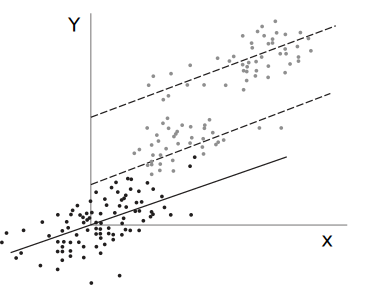
\includegraphics[scale=1]{images/fixed_effects_example.pdf}
\caption{Ejemplo de datos de diferentes sujetos}
\label{fig:efectos_fijo}
\end{figure}



\newcommand{\slopeestim}[1] { $\estslope \sim #1$ }

El modelo agrupado o pooled que vimos en el anterior capítulo ignora la posibilidad de heterogeneidad no observada; esto es, variables no medidas que afectan al sistema planteado. En el caso concreto de nuestro corpus, dicha heterogeneidad puede deberse a factores como la identidad o el género de los hablantes.

Los modelos de efectos fijos nos ayudan a controlar la heterogeneidad no observada cuando ésta es constante en el tiempo, dado un sujeto del sistema. Asumimos que estos factores son inherentes a la conversación entre el hablante y su interlocutor. Para este modelo, definimos los sujetos (en el lenguaje del modelo estadístico) como cada uno de los hablantes y sus respectivas sesiones. No nos importa si el mismo sujeto se repite en otra sesión: cada hablante de una sesión es un sujeto distinto para el modelo de efectos fijos.

Recordemos que el entrainment medido mediante el proceso TAMA es un proceso direccional: medimos la influencia de un hablante sobre el otro y viceversa. Así que el \entrainment de cada fila de nuestro set de datos (definido en la Sección \ref{sec:panel_data}) corresponde al valor de mimetización direccional del actual hablante sobre su par.


\section{Modelo de efectos fijos \emph{within group}}

Existen (al menos) dos variantes del modelo de efectos fijos: el modelo de variables ficticias y el modelo ``dentro del grupo'' (\emph{within group}). Ambas técnicas son matemáticamente equivalentes, pero utilizaremos la segunda que nos provee el estimador de la pendiente, que es lo único que nos interesa.

La técnica utilizada consiste en, dentro de cada grupo, restarle tanto a la variable ``dependiente'' como a la ``independiente'' las medias dentro de cada grupo (de aquí proviene el nombre del método). Esto resulta en ``sacarle'' los efectos fijos no-temporales: en nuestro caso, estos están contemplados dentro de la ordenada al origen. Luego de efectuar esta transformación, se aplica regresión lineal ``pooled'', como en el análisis anterior. Producto del pre-procesamiento de los datos, la ordenada al origen es negligible. En \cite[chap 16]{gujarati1999} se describe extensamente este procedimiento.


\section{Resultados}


\begin{table}[t!]
\begin{figure}[ht]
\centering
% psl is "Positive Slope"
\newcommand{\psl} { $+$ }
\newcommand{\ppsl} { $++$ }
\newcommand{\pppsl} { $+++$ }

% nsl stands for "Negative SLope"
\newcommand{\nsl} { $-$ }
\newcommand{\nnsl} { $--$ }
\newcommand{\nsl} { $---$ }


\begin{tabular}{| c | c | c | c | c | c |}
  \hline
               &\ENGMAX  & \ENGMEAN  & \FOMEAN  & \FOMAX  & NOISERATIO  \\
  \hline
  contributes  &         &           & \psl     &         & \psl        \\ \hline
  clear        & \pppsl  &           & \psl     &         & \psl        \\ \hline
  engaged      &         &           & \psl     &         &             \\ \hline
  planning     &         &           &          &         &             \\ \hline
  encourages   &         &           &          &         &             \\ \hline
  difficult    & \nsl    &           &          &         &             \\ \hline
  bored        &         &           & \nsl     &         &             \\ \hline
  dislikes     &         &           &          &         &             \\ \hline
  \hline
& PHON\_AVG & PHON\_COUNT & SHIMMER & SYL\_AVG & SYL\_COUNT \\
  \hline
contributes  &      &  &  &  &        \\ \hline
  clear      & \psl &  &  &  & \psl   \\ \hline
  engaged    &      &  &  &  &        \\ \hline
  planning   &      &  &  &  &        \\ \hline
  encourages &      &  &  &  &        \\ \hline
  difficult  &      &  &  &  &        \\ \hline
  bored      &      &  &  &  &        \\ \hline
  dislikes   &      &  &  &  &        \\ \hline
  \hline
\end{tabular}


\caption{Tabla que representa los resultados significantes del experimento. En una de las entradas, tenemos los nombres abreviados de las variables sociales, y en la otra las variables a/p. El símbolo \psl representa valor significante y positivo de la pendiente de la regresión de efectos fijos, mientras que \nsl representa significante y negativo }

\label{sign_table}

\end{figure}

\caption{Tabla que representa los resultados significantes del análisis. En una de las entradas, tenemos los nombres abreviados de las variables sociales, y en la otra las variables a/p. El símbolo \psl representa valor significante y positivo de la pendiente de la regresión de efectos fijos, mientras que \nsl representa significante y negativo }
\label{sign_table}
\end{table}

Este modelo, utilizando como variable independiente al valor absoluto del \entrainment dio valores sustancialmente apreciables. Casi todas las variables \ap poseen al menos un valor significativo de $\estslope$, destacándose \ENGMEAN, \NOISETOHARMONICS y \FOMEAN  con 3, 3 y 4 valores significativos respectivamente. En las Tablas \ref{fig:efectos_fijos_tabla1} y \ref{fig:efectos_fijos_tabla2} podemos ver el test de coeficientes con las variables sociales significativas resaltadas en distintas tonalidades según su nivel de significancia. Una versión simplificada tabla la podemos ver en la tabla \ref{sign_table} que grafica mediante tabla de doble entrada aquellos pares de variables \ap y variables sociales con coeficientes significativos y su signo.

Con respecto a las variables sociales, podemos observar que:

\begin{itemize}
  \item \svcontributes se relaciona positivamente con el \absentrainment cuando la variable acústico-prosódica medida es \FOMEAN o bien \NOISETOHARMONICS. Esto significa que, cuando sube el valor absoluto del \entrainment, esta variable positiva también lo hace con buena probabilidad. Esto es un efecto esperable: cuando hay mimetización, hay colaboración para el éxito en el juego.
  \item \svclear, otra variable que refleja una visión positiva del juego, también se relaciona positivamente con el \absentrainment para las variables \FOMEAN, \NOISETOHARMONICS, \ENGMAX como a su vez para \PHONAVG
  \item \svengaged, de la misma manera que las dos anteriores, relaciona positivamente pero sólo con \FOMEAN
  \item \svdifficult, se relaciona de la manera esperada con el \absentrainment cuando la variable acústico prosódica es \ENGMAX; esto es, con $\estslope < 0$. Esto tiene sentido, ya que a mayor mimetización de los interlocutores, la dificultad de estos para hablar debería disminuir. Por otro lado, $\estslope > 0$ cuando la variable acústico-prosódica es \ENGMEAN, lo cual no era un resultado esperado, pero bien puede ser parte del error estadístico.
  \item La variable \svbored se comporta de idéntica manera, sólo que con \FOMEAN.
  \item \svplanning y \svencourages, otras variables positivas, no presentan valores significativos.
  \item \svdislikes no presenta valores significativos
\end{itemize}


En resumen, encontramos fuerte evidencia empírica en favor de la hipótesis de que el valor absoluto del \entrainment se relaciona de manera positiva con atributos sociales de características positivas, mientras que lo hace de manera inversa con los que tienen connotaciones negativas.

Un hecho a destacar es que esta medida del entrainment es consistente con otras métricas definidas en otros trabajos, como las construídas en \cite{gravano2015backward} sobre anotaciones discretas de los patrones entonacionales usando la convención ToBI\cite{pitrelli1994evaluation}.

\begin{figure}[p]
\centering
\adjustbox{max width=\textwidth}{
\begin{tabular}{rrrrr}
  \hline
\ENGMAX & $\estslope$ & Std. Error & t value & Significance \\
  \hline
contributes\_to\_successful\_completion & 0.0720 & 0.4258 & 1.689631E-01 & 0.8660 \\
  \stronghl making\_self\_clear & 1.6914 & 0.3820 & 4.427376E+00 & 0.0000 \\
  engaged\_in\_game & 0.3456 & 0.2528 & 1.367266E+00 & 0.1732 \\
  planning\_what\_to\_say & 0.5655 & 0.5208 & 1.085851E+00 & 0.2790 \\
  gives\_encouragement & 0.4739 & 0.3744 & 1.265523E+00 & 0.2073 \\
  \stronghl difficult\_for\_partner\_to\_speak & -0.6925 & 0.2863 & -2.418510E+00 & 0.0166 \\
  bored\_with\_game & 0.2110 & 0.2543 & 8.298495E-01 & 0.4077 \\
  dislikes\_partner & -0.4254 & 0.3438 & -1.237312E+00 & 0.2175 \\

  \hline
\ENGMEAN & $\estslope$ & Std. Error & t value & Significance \\
  \hline
  \softhl contributes\_to\_successful\_completion & 0.6552 & 0.3610 & 1.814712E+00 & 0.0712 \\
  making\_self\_clear & 0.9470 & 0.6080 & 1.557502E+00 & 0.1211 \\
  \softhl engaged\_in\_game & 0.7091 & 0.3847 & 1.843187E+00 & 0.0669 \\
  planning\_what\_to\_say & 0.3636 & 0.5756 & 6.316937E-01 & 0.5284 \\
  gives\_encouragement & 0.4051 & 0.3482 & 1.163506E+00 & 0.2461 \\
  \hl difficult\_for\_partner\_to\_speak & 0.5287 & 0.2515 & 2.101960E+00 & 0.0369 \\
  bored\_with\_game & -0.0036 & 0.4106 & -8.663987E-03 & 0.9931 \\
  dislikes\_partner & 0.5307 & 0.3889 & 1.364514E+00 & 0.1741 \\

  \hline
\FOMEAN & $\estslope$ & Std. Error & t value & Significance \\
  \hline
  \stronghl contributes\_to\_successful\_completion & 0.9752 & 0.3058 & 3.188448E+00 & 0.0017 \\
  \softhl making\_self\_clear & 0.6998 & 0.3907 & 1.791239E+00 & 0.0749 \\
  \stronghl engaged\_in\_game & 0.8538 & 0.2773 & 3.078945E+00 & 0.0024 \\
  planning\_what\_to\_say & 0.6430 & 0.5363 & 1.198966E+00 & 0.2321 \\
  gives\_encouragement & 0.0006 & 0.3885 & 1.577445E-03 & 0.9987 \\
  difficult\_for\_partner\_to\_speak & -0.5323 & 0.3835 & -1.388190E+00 & 0.1667 \\
  \stronghl bored\_with\_game & -0.7663 & 0.2582 & -2.968508E+00 & 0.0034 \\
  dislikes\_partner & 0.0688 & 0.3808 & 1.806265E-01 & 0.8569 \\

\FOMAX & $\estslope$ & Std. Error & t value & Significance \\
  \hline
  \softhl contributes\_to\_successful\_completion & 0.7628 & 0.4381 & 1.741129E+00 & 0.0833 \\
  making\_self\_clear & 0.6718 & 0.4129 & 1.626984E+00 & 0.1054 \\
  engaged\_in\_game & 0.5308 & 0.3776 & 1.405582E+00 & 0.1615 \\
  planning\_what\_to\_say & 0.0489 & 0.4210 & 1.161167E-01 & 0.9077 \\
  gives\_encouragement & 0.4724 & 0.5464 & 8.647145E-01 & 0.3883 \\
  difficult\_for\_partner\_to\_speak & -0.3208 & 0.2821 & -1.136927E+00 & 0.2570 \\
  bored\_with\_game & -0.2584 & 0.3764 & -6.865032E-01 & 0.4933 \\
  dislikes\_partner & 0.1249 & 0.3884 & 3.216226E-01 & 0.7481 \\
\end{tabular}}

\caption{Tablas con los resultados de la regresión de efectos fijos sobre el va,or absoluto de \entrainment para \ENGMAX, \ENGMEAN, \FOMEAN y \FOMAX. En la segunda columna se cita el valor de $\estslope$, la desviación estándar calculada, el t-valor obtenido y la significancia. Las columnas resaltadas corresponden a aquellas significantes, con diferentes matices de gris según $p < 0.10$, $p < 0.5$, o $p < 0.01$}
\label{fig:efectos_fijos_tabla1}

\end{figure}




\begin{figure}[pt!]
\centering
\adjustbox{max width=\textwidth}{
\begin{tabular}{rrrrr}
  \hline
  \hline
\NOISETOHARMONICS & $\estslope$ & Std. Error & t value & Significance \\
  \hline
  \hl contributes\_to\_successful\_completion & 0.7271 & 0.3439 & 2.114275E+00 & 0.0358 \\
  \stronghl making\_self\_clear & 1.3576 & 0.3613 & 3.758007E+00 & 0.0002 \\
  engaged\_in\_game & 0.1270 & 0.3431 & 3.702043E-01 & 0.7117 \\
  planning\_what\_to\_say & -0.1625 & 0.4264 & -3.811856E-01 & 0.7035 \\
  gives\_encouragement & 0.7665 & 0.4860 & 1.577201E+00 & 0.1165 \\
  difficult\_for\_partner\_to\_speak & -0.1683 & 0.3400 & -4.951813E-01 & 0.6211 \\
  \softhl bored\_with\_game & 0.5527 & 0.3084 & 1.792251E+00 & 0.0747 \\
  dislikes\_partner & 0.3457 & 0.3279 & 1.054410E+00 & 0.2931 \\
   \hline

  \hline
\PHONAVG & $\estslope$ & Std. Error & t value & Significance \\
  \hline
contributes\_to\_successful\_completion & 0.5557 & 0.3577 & 1.553747E+00 & 0.1220 \\
  making\_self\_clear & 0.7598 & 0.5085 & 1.494093E+00 & 0.1369 \\
  engaged\_in\_game & 0.2440 & 0.2586 & 9.438356E-01 & 0.3465 \\
  planning\_what\_to\_say & 0.3614 & 0.5174 & 6.984626E-01 & 0.4858 \\
  gives\_encouragement & 0.0604 & 0.3829 & 1.576928E-01 & 0.8749 \\
  \softhl difficult\_for\_partner\_to\_speak & -0.6264 & 0.3374 & -1.856257E+00 & 0.0650 \\
  bored\_with\_game & -0.0158 & 0.3204 & -4.921947E-02 & 0.9608 \\
  dislikes\_partner & 0.0975 & 0.3137 & 3.108070E-01 & 0.7563 \\
   \hline

\SYLAVG & $\estslope$ & Std. Error & t value & Significance \\
  \hline
  contributes\_to\_successful\_completion & 0.2451 & 0.3663 & 6.692398E-01 & 0.5042 \\
  \softhl making\_self\_clear & 0.7934 & 0.4094 & 1.937743E+00 & 0.0542 \\
  engaged\_in\_game & 0.4956 & 0.3642 & 1.360687E+00 & 0.1753 \\
  planning\_what\_to\_say & 0.4429 & 0.5189 & 8.535430E-01 & 0.3945 \\
  gives\_encouragement & 0.2363 & 0.4192 & 5.637211E-01 & 0.5736 \\
  difficult\_for\_partner\_to\_speak & 0.1856 & 0.3481 & 5.332959E-01 & 0.5945 \\
  bored\_with\_game & -0.2909 & 0.3606 & -8.067536E-01 & 0.4208 \\
  dislikes\_partner & 0.1768 & 0.3452 & 5.120454E-01 & 0.6092 \\
   \hline

  \hline
\LOCALJITTER & $\estslope$ & Std. Error & t value & Significance \\
  \hline
contributes\_to\_successful\_completion & 0.5770 & 0.3759 & 1.534821E+00 & 0.1265 \\
  making\_self\_clear & 0.5057 & 0.4881 & 1.036143E+00 & 0.3015 \\
  \hl engaged\_in\_game & 0.4972 & 0.2515 & 1.977130E+00 & 0.0495 \\
  planning\_what\_to\_say & -0.0417 & 0.4628 & -9.000210E-02 & 0.9284 \\
  gives\_encouragement & -0.0160 & 0.3502 & -4.554031E-02 & 0.9637 \\
  difficult\_for\_partner\_to\_speak & -0.2788 & 0.3126 & -8.917922E-01 & 0.3737 \\
  bored\_with\_game & 0.1233 & 0.3155 & 3.906725E-01 & 0.6965 \\
  dislikes\_partner & -0.1171 & 0.2788 & -4.198582E-01 & 0.6751 \\
  \hline
\LOCALSHIMMER & $\estslope$ & Std. Error & t value & Significance \\
  \hline
contributes\_to\_successful\_completion & 0.3745 & 0.2754 & 1.359709E+00 & 0.1756 \\
  making\_self\_clear & -0.0097 & 0.3821 & -2.544762E-02 & 0.9797 \\
  engaged\_in\_game & 0.2434 & 0.2881 & 8.449092E-01 & 0.3993 \\
  planning\_what\_to\_say & -0.6040 & 0.4735 & -1.275476E+00 & 0.2037 \\
  \softhl gives\_encouragement & 0.3638 & 0.2057 & 1.768094E+00 & 0.0787 \\
  difficult\_for\_partner\_to\_speak & 0.2707 & 0.2720 & 9.952034E-01 & 0.3209 \\
  bored\_with\_game & -0.3635 & 0.2772 & -1.311203E+00 & 0.1914 \\
  dislikes\_partner & -0.1895 & 0.2667 & -7.105564E-01 & 0.4783 \\
\end{tabular}}

\caption{Tablas con los resultados de la regresión de efectos fijos para \NOISETOHARMONICS, \SYLAVG, \PHONAVG, \LOCALSHIMMER y \LOCALJITTER. En la segunda columna se cita el valor de $\estslope$, la desviación estándar calculada, el t-valor obtenido y la significancia. Las columnas resaltadas corresponden a aquellas significantes, con diferentes matices de gris según $p < 0.10$, $p < 0.5$, o $p < 0.01$}

\label{fig:efectos_fijos_tabla2}
\end{figure}



\chapter{Conclusiones y trabajo futuro}
\begin{frame}
\frametitle{Conclusiones}

\begin{enumerate}
  \item Desarrollo de métrica de entrainment automática a partir de conversaciones transcritas.
  \item Indicios de validación de la métrica introducida por Kousidis et al en un corpus orientado a tareas.
  \item Más indicios sobre la prevalencia y característica positiva del disentrainment
\end{enumerate}


\end{frame}

\begin{frame}
\frametitle{Trabajo a futuro}

\begin{enumerate}
  \item Reproducir experimentos sobre otros corpus, por ejemplo Switchboard \footnote{https://catalog.ldc.upenn.edu/LDC97S62}
  \item Chequear filtro de prewhitening
  \item Análisis multivariado de las variables \ap para construir nuevas métricas de entrainment
\end{enumerate}
\end{frame}


\chapter{Apéndice}
\section{Series de Tiempo}

En términos informales, una serie de tiempo es un conjunto de datos recolectados a través del tiempo.



%%%% BIBLIOGRAFIA
\chapter{Bibliografía}
\backmatter

\bibliographystyle{alpha}
\bibliography{tesis}
\end{document}
